\documentclass{article}

\usepackage[style=numeric]{biblatex}
\usepackage{graphicx}

\renewcommand{\abstractname}{Resumen}
\renewcommand{\refname}{Bibliografía}
\setlength{\parskip}{1em}
\setlength{\parindent}{0em}

\begin{document}

\title{COMBINANDO VISIÓN ARTIFICIAL Y MODELOS DE LENGUAJE PARA INTERPRETACIÓN DE LENGUA DE SEÑAS CHILENA (LSCh)}

\author{Cristóbal Fajardo, Pablo Gaete, Rubén Torres \\ 
Profesor Guía: Juan Bekios}


\maketitle


\begin{abstract}

La escasez de intérpretes de Lengua de Señas Chilena (LSCh), especialmente en el ámbito de la salud, representa un desafío significativo para las personas sordas en Chile, dificultando el acceso a un tratamiento adecuado particularmente en el área de la salud mental. En este trabajo, se propone una solución digital que ofrece una alternativa accesible y de menor costo en comparación con los intérpretes profesionales. Nuestra propuesta combina la detección de puntos clave de las manos (hand landmark detection) con redes neuronales LSTM, complementadas por un modelo de lenguaje de gran escala (LLM) para lograr una mayor fluidez al transformar señas individuales en oraciones completa

El sistema ha demostrado una tasa de acierto del 92.5\% en el reconocimiento de palabras individuales y una similitud del 96.35\% comparado con las frases esperadas (utilizando la distancia de Levenshtein) en la traducción de frases completas. Además, utiliza una arquitectura cliente-servidor, que asegura escalabilidad y accesibilidad desde dispositivos con recursos limitados. A pesar de estos resultados prometedores, áreas como la ampliación del dataset y la reducción de latencia siguen siendo desafíos clave para el desarrollo futuro.

Esta solución digital no solo tiene el potencial de mejorar el acceso de las personas sordas en Chile a servicios críticos, sino que también abre nuevas oportunidades para la investigación y el desarrollo de tecnologías inclusivas en el ámbito de la comunicación asistida.

\end{abstract}

\section{Introducción}

\subsection{Descripción del problema}

En Chile, el II Estudio Nacional de la Discapacidad realizado por el Ministerio de Desarrollo Social y SENADIS en 2015 \cite{cita12}, el 16,7\% de la población presenta algún tipo de discapacidad, equivalente a 2.836.818 personas. De estas, el 3,6\% tiene dificultades auditivas, lo que representa aproximadamente 611.000 personas, de las cuales 180.000 padecen sordera total \cite{cita1}.

La escasez de intérpretes de Lengua de Señas genera una significativa exclusión de las personas sordas en nuestra sociedad, una situación particularmente evidente en el ámbito de la salud, uno de los pilares fundamentales para el bienestar humano.
En el ámbito de la salud mental, las personas sordas enfrentan una exclusión sistemática debido a la falta de comunicación efectiva con los profesionales, lo que incrementa los riesgos de exclusión social y dificulta su bienestar. Esta problemática resalta la necesidad urgente de soluciones tecnológicas que puedan abordar estas brechas de accesibilidad.

\subsection{Hipótesis de trabajo}

La implementación de un modelo de interpretación del Lenguaje de Señas Chileno (LSCh)
utilizando detección de manos con landmarks y redes neuronales LSTM, combinado con un
modelo de lenguaje (LLM) puede alcanzar una tasa de acierto mayor al 90\%, con un costo menor y una disponibilidad mayor que un intérprete humano.

\subsection{Objetivos}

Lorem ipsum dolor sit amet

\subsubsection{General}

Lorem ipsum dolor sit amet

\subsubsection{Específicos}

Lorem ipsum dolor sit amet

\section{Estado del arte}

Lorem ipsum dolor sit amet

\subsection{Discusión Bibliográfica}

Lorem ipsum dolor sit amet

\subsection{Marco Teórico}

Lorem ipsum dolor sit amet

\section{Modelo Propuesto: LSTM + Hand landmarker + LLM}

En esta sección se describe el modelo a utilizar para probar la hipótesis. A diferencia de los modelos SVG o YOLO, discutidos en el capítulo 2.1, la red LSTM puede capturar datos históricos de la secuencia de imágenes para poder interpretar señas y gestos de manera dinámica. Para el entrenamiento, se utilizarán datos de hand landmarks derivados del conjunto de datos original, de esta manera se descarta parte del ruido y se sintetiza información relevante.

Utilizando este mecanismo se pueden identificar gestos que corresponden a palabras o frases individuales. Al agrupar listas de palabras que forman una oración, el siguiente paso consiste en usarlas como entrada al LLM gpt-3.5-turbo, junto con un prompt que permita obtener una frase con la fluidez propia del lenguaje hablado.

\subsection{Arquitectura del sistema}

La arquitectura propuesta está compuesta por tres componentes principales. El primero, una capa de MediaPipe hand landmarker, para obtener la lista de coordenadas de los puntos clave para cada mano.

El segundo componente es una red LSTM, que combina capas bidireccionales LSTM y densas para procesar datos secuenciales. La primera capa LSTM bidireccional captura patrones temporales en ambas direcciones y devuelve secuencias completas para la siguiente capa. La segunda LSTM bidireccional resume la información en una representación compacta. Luego, una capa densa con 128 neuronas y activación ReLU permite aprender relaciones no lineales, seguida de un Dropout del 50% para evitar sobreajuste. Finalmente, una capa densa con activación softmax produce probabilidades para las clases objetivo.

El tercer componente consiste en utilizar gpt-3.5-turbo, para derivar oraciones fluidas, dada una lista de palabras, y el prompt “Convierte la siguiente secuencia de palabras de lengua de señas chilena a una frase en español coherente”

\begin{figure}[!hbtp]
    \centering
    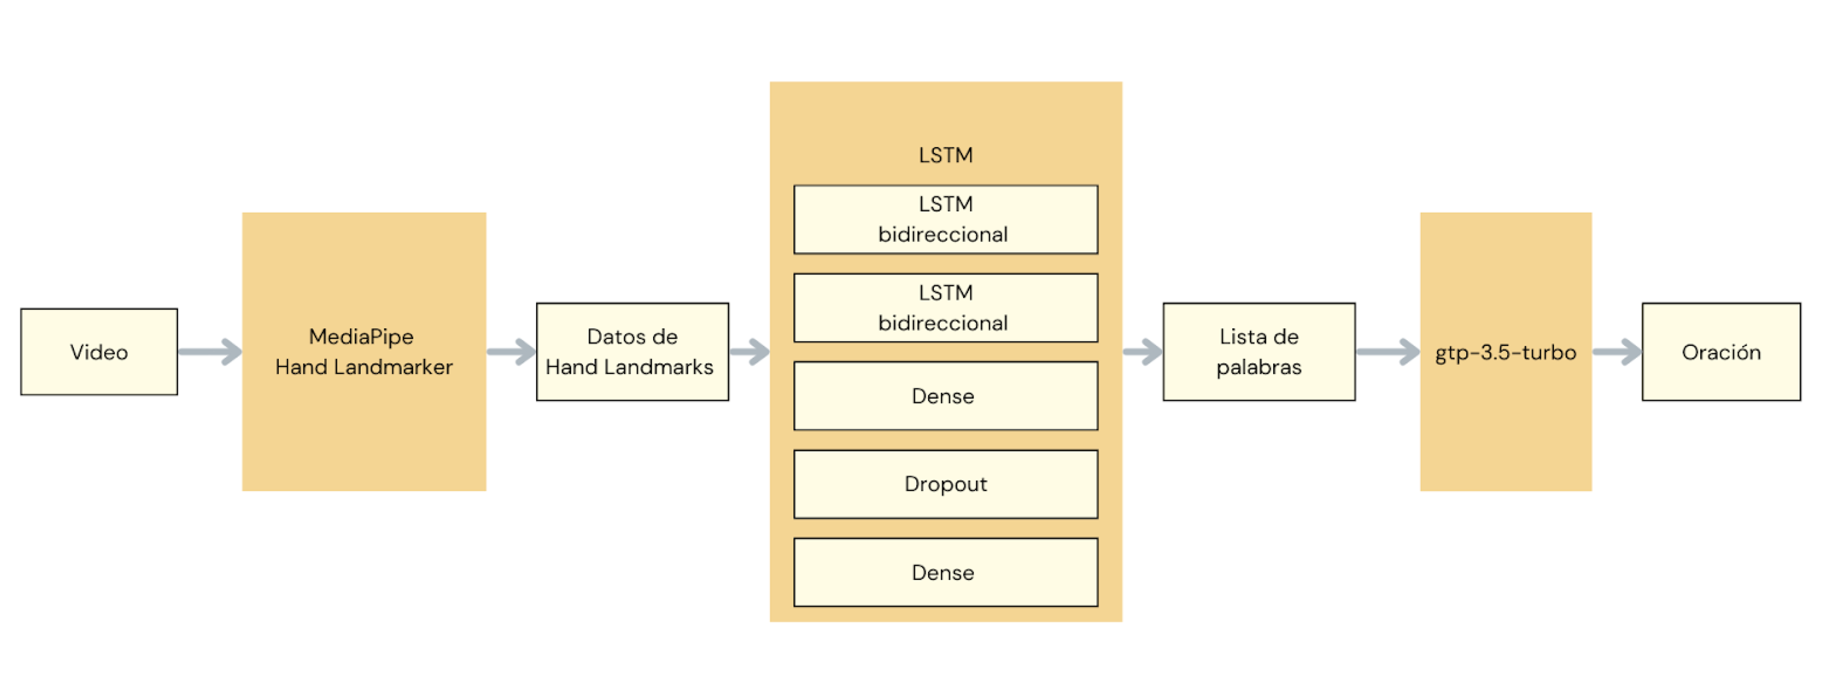
\includegraphics[width=5in]{figuras/architecture-diagram.png}
		\caption{Diagrama de bloques de la arquitectura propuesta}
		\label{fig1}
\end{figure}

\section{Experimentos}

Lorem ipsum dolor sit amet

\section{Resultados}

Lorem ipsum dolor sit amet


\section{Conclusiones}

En el presente trabajo se ha realizado una revisión del estado del arte de los métodos para interpretar la Lengua de señas Chilena, así como otros métodos utilizados internacionalmente, proponiendo una solución que combina diferentes modelos para obtener un resultado con una tasa de acierto y porcentaje de coincidencia de las traducciones finales, sobre 90\%, en el contexto de una arquitectura cliente-servidor que permita su ejecución desde dispositivos portátiles, en particular de baja y media gama, con una latencia en el orden de los 1 a 2 segundos.


De estos resultados podemos concluir que este esquema tiene potencial para permitir la accesibilidad de las personas sordas a los servicios de salud, sin necesidad de un intérprete. Sin embargo, aún quedan grandes retos por resolver. Por un lado, es necesario recopilar un conjunto de datos robusto y representativo de la Lengua de Señas Chilena, ya que los datos actuales son muy limitados y no abarcan la diversidad de señas necesarias para aplicaciones generalizadas. Por otro lado, reducir la latencia a menos de un segundo, mejoraría significativamente la calidad de la comunicación, permitiendo interacciones más fluidas.


\begin{thebibliography}{99}

\bibitem{cita1}  Herrera, M. (2023, Febrero) Falta de inclusión, estigma social y discriminación: la compleja realidad diaria que vive una persona sorda en Chile. La Tercera. Santiago. p. 1 

\bibitem{cita2} Mendía R. y García C. (2021, Enero). Comunidad sorda y salud mental: Un abandono silencioso. La Tercera. Santiago. p. 1

\bibitem{cita3} Gonzalez, C. y Yimes F. (2016) Sistema de reconocimiento gestual de lengua de señas chilena mediante cámara digital p. 36-41

\bibitem{cita4} Acuña, X., Adamo, D. y Cabrera I. (2009) Diccionario Bilingüe de Lengua de Señas Chilena-Español. p. 17-18

\bibitem{cita5} Andrare, L. y Catril, R. (2022) Reconocimiento en tiempo real del alfabeto de lengua de señas chilena empleando aprendizaje automático. p. 53-62

\bibitem{cita6} Pathan, R. K., Biswas, M., Yasmin, S., Khandaker, M. U., Salman, M., \& Youssef, A. A. F. (2023). Sign language recognition using the fusion of image and hand landmarks through multi-headed convolutional neural network. p. 4-9

\bibitem{cita7}  Bala, D., Sarkar, B., Abdullah, M. I., \& Hossain, M. A. (2021). American Sign Language alphabets recognition using convolutional neural network. International Journal of Knowledge Based Computer Systems.

\bibitem{cita8}  Makkar, A., Makkar, D., Patel, A., \& Hebert, L. (2024). SignSpeak: Open-source time series classification for ASL translation.

\bibitem{cita9}  Renjith, S., \& Manazhy, R. (2024). Sign language: A systematic review on classification and recognition. P. 14-15

\bibitem{cita10} Gong, J., Foo, L. G., He, Y., Rahmani, H., \& Liu, J. (2024). LLMs are good sign language translators. 

\bibitem{cita11} Imran, A., Hulikal, M. S., \& Gardi, H. A. A. (2024). Real Time American Sign Language Detection Using YOLO-v9

\bibitem{cita12} Ministerio de Desarrollo Social y Servicio Nacional de la Discapacidad (SENADIS). (2015). II Estudio Nacional de la Discapacidad.


\end{thebibliography}

\end{document}
